\documentclass[10pt]{article}

% Define margins
\setlength{\topmargin}{-1.0cm}
\setlength{\oddsidemargin}{0.1cm}
\setlength{\textwidth}{16.5cm}
\setlength{\textheight}{23.0cm}

% Packages
\usepackage{url}
\usepackage[hidelinks]{hyperref}
\usepackage{subfig}
\usepackage{graphicx}
\usepackage{comment}

% Color
\usepackage{xcolor}
\newcommand{\magenta}[1]{\textcolor{magenta}{#1}}
\newcommand{\red}[1]{\textcolor{red}{#1}}
\newcommand{\blue}[1]{\textcolor{blue}{#1}}
\newcommand{\green}[1]{\textcolor{green}{#1}}


% Long version
\newif\iflongproposal
\longproposaltrue % comment out for a short proposal



\begin{document}
	\begin{center}
		\large\textbf{Research Statement} 
	\end{center}
	\textbf{Bishwamittra Ghosh}\\		
	\noindent Scientist\\
	IHPC, A*STAR, Singapore\\
	\blue{\url{https://bishwamittra.github.io}}



	\paragraph{}
	My research is on fairness and explainability in machine learning applied in safety-critical domains. Traditional machine learning, particularly deep learning, is known for  unfair predictions towards marginalized sensitive groups and for generating black-box predictions. In my research, I design algorithmic framework to \textit{formally quantify fairness in machine learning}~\cite{ghosh2021justicia, ghosh2022algorithmic}, \textit{explain the sources of unfairness}~\cite{ghosh2022how}, and \textit{learn explainable rule-based classifiers}~\cite{ghosh22efficient, ghosh2019incremental, ghosh2020classification}. Prior approaches to these problems are often limited by scalability, accuracy, or both. To address the limitations, I closely integrate automated reasoning, formal methods, and statistics with fairness and explainability to develop scalable and accurate solutions.
	
	

	
	
	During my PhD, I have  research collaborations and internships in academia and industry. In addition to fairness and explainability, I have collaborative research on  group testing~\cite{ciampiconi2020maxsat}, social-spatial group queries~\cite{ghosh2018flexible, apon2021social}, and hypergraph core decomposition~\cite{arafat2023neighborhood}. We publish our research in leading conferences and journals in artificial intelligence and machine learning (AAAI-$22$, $21$, $20$, JAIR-$22$, FAccT-$ 23 $, ECAI-$20$, AIES-$19$) and databases (VLDB-$23$, $18$, TSAS-$2022$).
	
	
	
	
	
%	\section*{Dissertation Research}
	
	\subsection*{Research Thrust 1: Fairness in Machine Learning}
	
	Fairness in machine learning focuses on quantifying and mitigating the unfairness or bias of the prediction of the classifier towards different sensitive groups in the data. To quantify bias in algorithmic decision-making, multiple fairness metrics have been proposed based on societal belief and norms. However, there has been insignificant progress in \textit{formally quantifying existing fairness metrics}. In addition, fairness metrics measure the overall bias of a classifier, but they cannot  \textit{explain the sources of bias}. Therefore, our research focuses on two key aspects: formally quantifying bias of a classifier and explaining its sources.
	
	\subsubsection*{Probabilistic Fairness Quantification} In probabilistic fairness quantification, we formally quantify the bias of a classifier given the distribution of input features\textemdash essentially beyond a finite dataset. We propose two approaches to the problem: a general approach for finite classifiers encoded as Boolean formulas~\cite{ghosh2021justicia} and a specific approach for linear classifiers~\cite{ghosh2022algorithmic}.
	

	
	
	\paragraph{Fairness Quantification via SSAT.} The key idea in quantifying group fairness metrics is to compute the maximum (resp.\ minimum) probability of predictions of the classifier across all sensitive groups\textemdash the probability of selecting White-male vs.\ Black-female candidates in job applications. We propose a stochastic satisfiability (SSAT) based framework, called $\mathsf{Justicia}$~\cite{ghosh2021justicia}, for computing such probabilities. 
	\iflongproposal
	More specifically, the maximum probability becomes the solution of an existential-random (ER)-SSAT formula\textemdash we encode the classifier as a Boolean formula, the feature distribution via random Boolean variables, and compute the maximum conditional probability of the satisfaction of the formula for existentially quantified sensitive features.
	\fi
	In the presence of multiple sensitive features resulting in exponentially many sensitive groups, SSAT efficiently finds the most (resp.\ least) favored
	\iflongproposal
	group by the classifier, thanks to the significant progress in satisfiability (SAT) solving, and particularly in weighted model counting problem.
	\else
	group.
	\fi 
	In experiments, $\mathsf{Justicia}$ is more scalable in the fairness quantification of tree-based classifiers than existing SMT or sampling methods.
	
	
	\paragraph{Tractable Fairness Quantification with Feature Correlation.} We extend $\mathsf{Justicia}$ to consider feature correlations for an accurate fairness quantification~\cite{ghosh2022algorithmic}. We consider a Bayesian network to represent the conditional distribution of 
	\iflongproposal
	features\textemdash the SSAT formula grows with the complexity of the Bayesian network, calling for a more scalable solution.	Therefore, we
	\else
	features and
	\fi
	demonstrate a tractable fairness quantification for linear classifiers by proposing stochastic subset sum 
	\iflongproposal
	problem, which admits an efficient dynamic programming solution with pseudo-polynomial complexity.
	\else
	problem.
	\fi 
	Experimentally, $\mathsf{Justicia}$ becomes more accurate and scalable than existing fairness verifiers for linear classifiers.
	
	
	
	
	
	\subsubsection*{Explaining Fairness Metrics: Identifying Sources of Bias}
	We combine both explainability and fairness in machine learning and propose a framework for explaining fairness.  We formalize \textit{fairness influence functions} (FIFs) to quantify the contribution of an individual feature and the intersection of multiple features to the resulting bias of the classifier~\cite{ghosh2022how}. 	Based on global sensitivity analysis, we propose a model-agnostic framework, called $\mathsf{FairXplainer}$, to estimate FIFs. 
	\iflongproposal
	The key idea is to represent fairness metrics using the variance of predictions and apply variance decomposition to compute FIFs.
	\fi
	In experiments, FIFs are highly correlated with fairness  
	\iflongproposal
	interventions and demonstrate a higher granular explanation of unfairness through intersectional influences,
	\else 
	interventions, 
	\fi
	unlike existing local explainability methods. In addition, $\mathsf{FairXplainer}$ approximates bias via FIFs with lower error than prior 
	\iflongproposal
	methods across classifiers such as neural networks and SVMs.
	\else
	methods.
	\fi
	
	

		
	
	\subsection*{Research Thrust 2: Explainable Rule-based Machine Learning}

	\red{interpret}able machine learning often employs rule-based classifiers, which use a set of rules to represent the decision boundary. The \red{interpret}ability of such classifiers depends on the size of the rules: smaller rules with higher accuracy are preferred in practice. However, this presents a challenge when dealing with large datasets, as \red{interpret}able classification learning becomes a combinatorial optimization problem that suffers from poor scalability. To address this issue, we propose an incremental learning framework for \red{interpret}able rule-based classification on large datasets. Our framework combines maximum satisfiability (MaxSAT) and mixed integer linear programming (MILP) with mini-batch learning.
	
	\subsubsection*{Scalability via Incremental Learning}
	We introduce a new incremental learning framework, referred to as $\mathsf{IMLI}$, which is based on MaxSAT for learning \red{interpret}able classification rules in propositional logic. The framework aims to optimize both the accuracy and \red{interpret}ability of the classification rules through a joint objective function, and an optimal rule is learned by solving a specially designed MaxSAT query. However, while MaxSAT has made considerable progress in the last decade, it is not scalable to practical classification datasets with thousands to millions of samples. To address this, we incorporate an efficient incremental learning technique that integrates mini-batch learning and iterative rule-learning within the MaxSAT formulation. This results in a framework that learns a classifier by iteratively covering the training data, solving a sequence of smaller MaxSAT queries corresponding to each mini-batch in each iteration. Our experiments demonstrate that $\mathsf{IMLI}$ achieves the best balance among prediction accuracy, \red{interpret}ability, and scalability, with competitive accuracy and \red{interpret}ability compared to existing \red{interpret}able classifiers, and impressive scalability on large datasets where both \red{interpret}able and non-\red{interpret}able classifiers fail. Finally, we apply $\mathsf{IMLI}$ to learn popular \red{interpret}able classifiers such as decision lists and decision sets.
	
	\subsubsection*{Expressiveness via Logical Relaxation}
	We extend our incremental learning framework to enable the learning of a more relaxed representation of classification rules with higher expressiveness, as described in~\cite{ghosh2020classification}. Specifically, we consider relaxed definitions of the standard OR/AND operators in propositional logic by allowing exceptions in the construction of a clause and in the selection of clauses in a rule. Based on these relaxed definitions, we introduce relaxed logical classification rules, which are motivated by the use of checklists in the medical domain and Boolean cardinality constraints. These rules generalize widely used rule representations, such as CNF, DNF, and decision sets. However, the combinatorial structure of these rules results in exponential succinctness, and na"ive learning techniques are computationally expensive. To overcome this issue, we propose an incremental mini-batch learning procedure, called $\mathsf{CRR}$, which leverages advances in MILP solvers to efficiently learn such rules. Our experimental analysis shows that $\mathsf{CRR}$ can generate more accurate and sparser classification rules compared to alternative rule-based classifiers.
	
	
	
	
%	\paragraph{Incremental Learning of \red{interpret}able Classfication Rules.} We propose an incremental learning framework, called $ \mathsf{IMLI} $~\cite{ghosh22efficient,ghosh2019incremental},  based on maximum satisfiability (MaxSAT) for synthesizing classification rules expressible in proposition logic. $ \mathsf{IMLI} $ considers a joint objective function to optimize the accuracy and the \red{interpret}ability of classification rules and learns an optimal rule by solving an appropriately designed MaxSAT query. Despite the progress of MaxSAT solving in the last decade, the straightforward MaxSAT-based solution cannot scale to practical classification datasets containing thousands to millions of samples. Therefore, we incorporate an efficient incremental learning technique inside the MaxSAT formulation by integrating mini-batch learning and iterative rule-learning. The resulting framework learns a classifier by iteratively covering the training data, wherein in each iteration, it solves a sequence of smaller MaxSAT queries corresponding to each mini-batch. In our experiments, $ \mathsf{IMLI} $ achieves the best balance among prediction accuracy, \red{interpret}ability, and scalability. For instance, $ \mathsf{IMLI} $ attains a competitive prediction accuracy and \red{interpret}ability w.r.t. existing \red{interpret}able classifiers and demonstrates impressive scalability on large datasets (Figure~\ref{fig:scalability_imli}) where both \red{interpret}able and non-\red{interpret}able classifiers fail. As an application, we deploy $ \mathsf{IMLI} $ in learning popular \red{interpret}able classifiers such as decision lists and decision sets.
	
	\begin{comment}
	\begin{figure}[!b]
		
		\centering
		
		\subfloat[Samples: $ 32,561 $\\Features: $ 94 $]{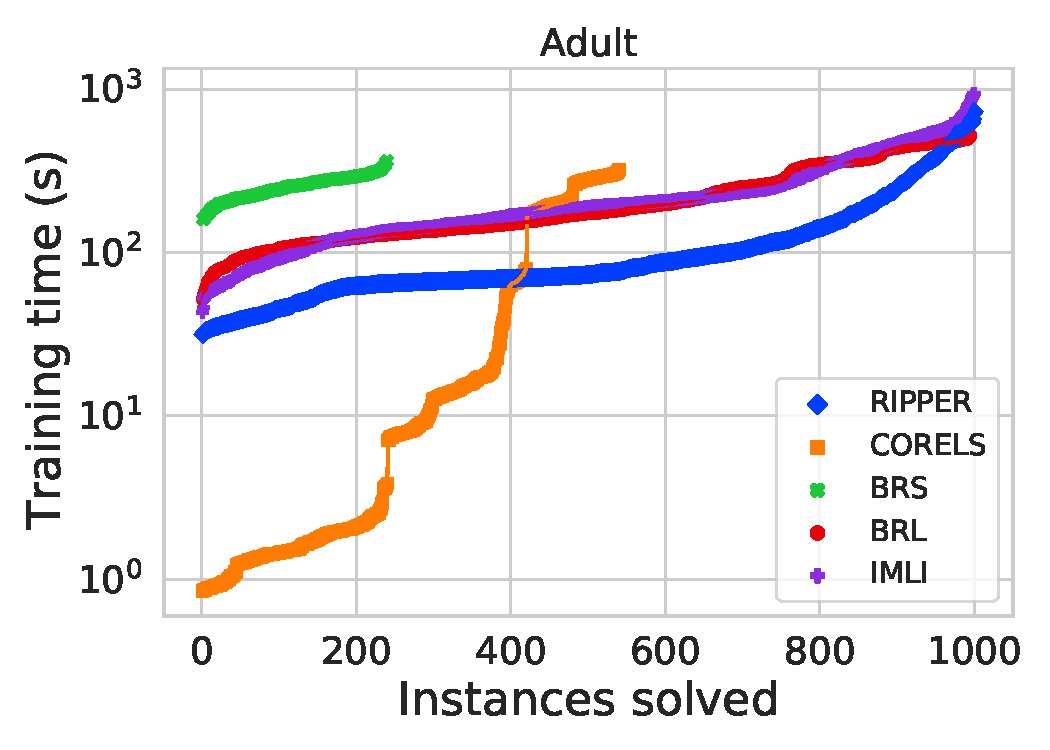
\includegraphics[scale=0.3]{figures/dataset_adult_cactus_train_val_fit_time}}
		\subfloat[Samples: $  107, 696 $\\Features: $ 169 $]{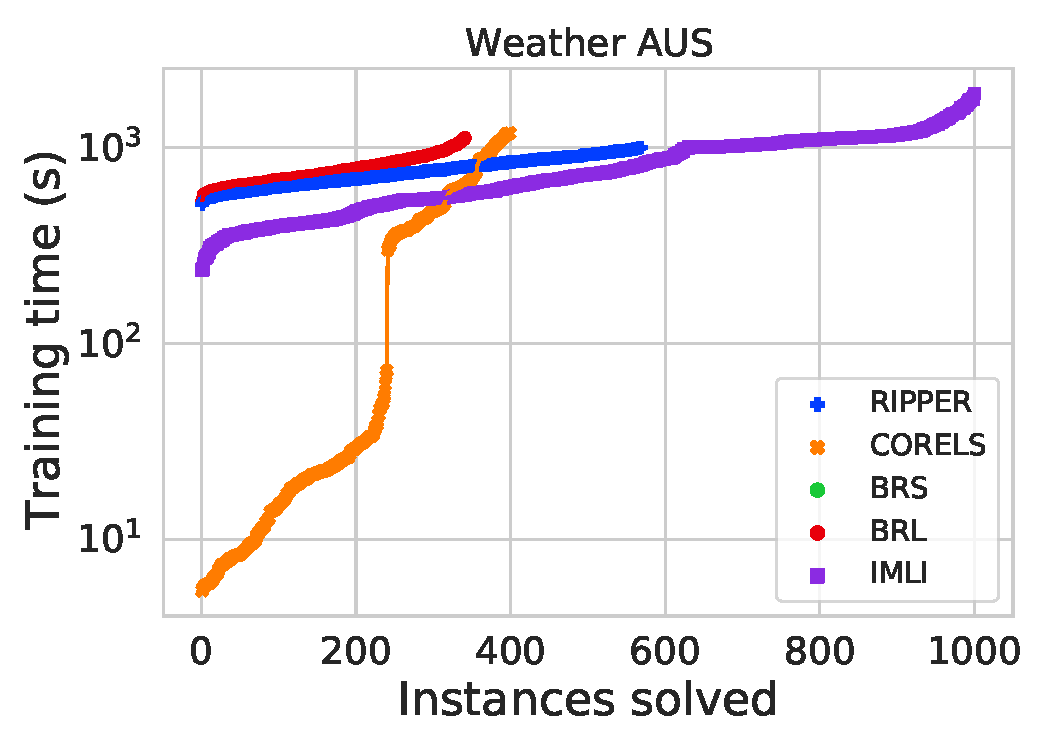
\includegraphics[scale=0.3]{figures/dataset_weatherAUS_cactus_train_val_fit_time}}
		\subfloat[Samples: $  1, 000, 000 $\\Features: $ 89 $]{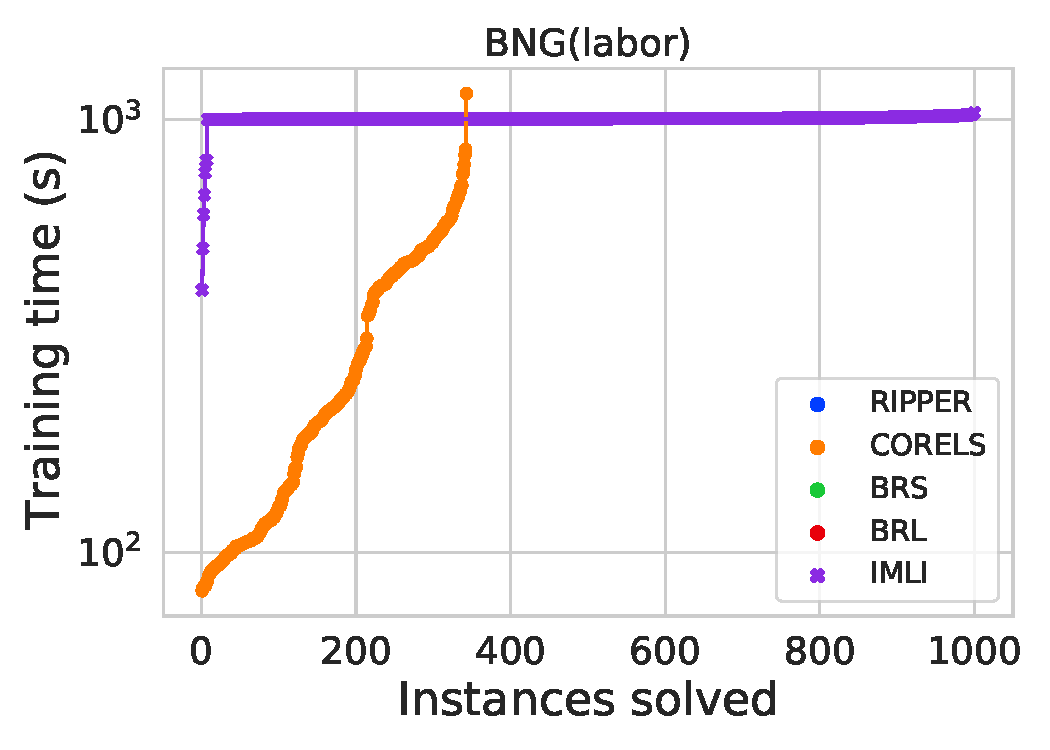
\includegraphics[scale=0.3]{figures/dataset_labor_cactus_train_val_fit_time}}
		
		\caption{Results on the scalability of $ \mathsf{IMLI} $ compared to existing \red{interpret}able classifiers, presented using cactus plots for datasets with varied dimensions. As datasets become large, $ \mathsf{IMLI} $ becomes the only \red{interpret}able classifier to classify all of $ 1000 $ classification instances for a dataset. The success of $ \mathsf{IMLI} $ is attributed to its incremental learning wrapping a MaxSAT-based formulation.}
		\label{fig:scalability_imli}
	\end{figure}
	\end{comment}
	
	
	
%	\paragraph{Classification Rules in Relaxed Logical Form.} We extend our incremental learning framework to learn a more relaxed representation of classification rules~\cite{ghosh2020classification}. Elaborately, we consider relaxed definitions of standard OR/AND operators in Boolean logic, which allow exceptions in the construction of a clause and also in the selection of clauses in a rule. Building on these relaxed definitions, we introduce relaxed-CNF classification rules motivated by the popular usage of checklists in the medical domain. Relaxed-CNF generalizes widely employed rule representations including CNF, DNF, and decision sets. While the combinatorial structure of relaxed-CNF rules offers exponential succinctness, the na\"ive learning techniques are computationally expensive. To this end, we propose an incremental mini-batch learning procedure, called $ \mathsf{CRR} $, that employs advances in the Mixed-Integer Linear Programming (MILP) solvers to efficiently learn relaxed-CNF rules. Our experimental analysis demonstrates that $ \mathsf{CRR} $ can generate relaxed-CNF rules, which are more accurate and sparser compared to the alternative rule-based models.
	
	

	
	\section*{Future Research Plans}
	 My long-term research plan is focused on designing efficient and scalable algorithms for machine learning, with a particular emphasis on their trustworthiness in safety-critical applications. To achieve this goal, I plan to work in a collaborative environment, where I can better understand the challenges arising in real-world applications and use advances in machine learning and formal methods to solve them. In pursuit of this vision, I have identified several key research themes that will guide my work.
	 
	 
	 \paragraph{Fairness and \red{interpret}ability As a Service.} I believe that in the future, machine learning will serve as an alternative decision-maker to humans in various domains, including law, education, and transportation. However, in high-stakes and safety-critical applications, black-box algorithms are expected to provide higher transparency. Therefore, it is crucial to achieve fairness, \red{interpret}ability, robustness, and privacy in machine learning models. However, traditional machine learning models, such as deep learning, are often data-hungry, making it challenging to certify and quantify properties such as fairness and \red{interpret}ability in complex models and large datasets. With this in mind, my research aims to develop efficient algorithms for ensuring the fairness and \red{interpret}ability of deep learning models, transformer-based natural language processing (NLP), and computer vision. 
	 
	 
	 \paragraph{Counting and Optimization Problems.} In my previous research, I focused on formulating fairness and \red{interpret}ability in machine learning as counting and optimization problems. I developed algorithms based on formal methods and incremental solving, which resulted in both higher scalability and better accuracy. Building on this work, I plan to extend these techniques to solve counting and optimization problems in areas beyond machine learning.
	
	\small
	\bibliographystyle{ieeetr}
	\bibliography{ref}
\end{document}